
% Beamer Presentation
% LaTeX Template
% Version 1.0 (10/11/12)
%
% This template has been downloaded from:
% http://www.LaTeXTemplates.com
%
% License:
% CC BY-NC-SA 3.0 (http://creativecommons.org/licenses/by-nc-sa/3.0/)
%
%%%%%%%%%%%%%%%%%%%%%%%%%%%%%%%%%%%%%%%%%

%----------------------------------------------------------------------------------------
%	PACKAGES AND THEMES
%----------------------------------------------------------------------------------------

\documentclass{beamer}
\usepackage[italian]{babel}
\usepackage{tikz}
\usetikzlibrary{arrows.meta}


\mode<presentation> {

% The Beamer class comes with a number of default slide themes
% which change the colors and layouts of slides. Below this is a list
% of all the themes, uncomment each in turn to see what they look like.

%\usetheme{default}
%\usetheme{AnnArbor}
%\usetheme{Antibes} 6
%\usetheme{Bergen}
%\usetheme{Berkeley}
%\usetheme{Berlin}
%\usetheme{Boadilla}
%\usetheme{CambridgeUS}
%\usetheme{Copenhagen} OK
%\usetheme{Darmstadt}
%\usetheme{Dresden}
%\usetheme{Frankfurt}
%\usetheme{Goettingen}
%\usetheme{Hannover}
%\usetheme{Ilmenau}
%\usetheme{JuanLesPins}
%\usetheme{Luebeck} OK
%\usetheme{Berlin} La migliore con le barre sopra
%\usetheme{Malmoe} Molto buona e più pulita
%\usetheme{Marburg}
%\usetheme{Montpellier}
%\usetheme{PaloAlto}
%\usetheme{Pittsburgh} ma a pittsburgh leggono da destra a sinistra? mah
\usetheme{metropolis} %top in versione minimal, copenhagen uguale (ma anni 80)
%\usetheme{Singapore} il gradiente non separa bene il titolo, boh
%\usetheme{Szeged} orrendo
%\usetheme{Warsaw} non malaccio, mix pittsburgh e copenhagen, anche se vorrei più titolo

%scelgo per ora 
% As well as themes, the Beamer class has a number of color themes
% for any slide theme. Uncomment each of these in turn to see how it
% changes the colors of your current slide theme.

\definecolor{amber}{HTML}{ffc400} % UBC Blue (primary)
\definecolor{dorange}{HTML}{ff3d00} % UBC Blue (primary)
\definecolor{orange}{HTML}{ff9100} % UBC Blue (primary)
\definecolor{black}{HTML}{000000} % UBC Blue (primary)

\setbeamercolor{palette primary}{bg=amber,fg=white}
\setbeamercolor{palette secondary}{bg=dorange,fg=white}
\setbeamercolor{palette tertiary}{bg=dorange,fg=white}
\setbeamercolor{palette quaternary}{bg=dorange,fg=white}
\setbeamercolor{structure}{fg=black} % itemize, enumerate, etc
\setbeamercolor{section in toc}{fg=dorange} % TOC sections

%\usecolortheme{albatross}
%\usecolortheme{beaver}
%\usecolortheme{beetle}
%\usecolortheme{crane}
%\usecolortheme{dolphin}
%\usecolortheme{dove}
%\usecolortheme{fly}
%\usecolortheme{lily}
%\usecolortheme{orchid}
%\usecolortheme{rose}
%\usecolortheme{seagull}
%\usecolortheme{seahorse}
%\usecolortheme{whale}
%\usecolortheme{wolverine}
}
\usepackage[utf8]{inputenc}
\usepackage[T1]{fontenc}
\usepackage{ae,aecompl,gensymb,textcomp} % Non fa i font pixeleschi nel pdf
\usepackage{graphicx} % Allows including images
\usepackage{booktabs} % Allows the use of \toprule, \midrule and \bottomrule in tables

%----------------------------------------------------------------------------------------
%	TITLE PAGE
%----------------------------------------------------------------------------------------

\title{\textbf{First Person Action Recognition}} % The short title appears at the bottom of every slide, the full title is only on the title page
\subtitle{Project Presentation}
\author{Nicolò Bertozzi \and Francesco Bianco Morghet} % Your name
\institute[Politecnico di Torino] % Your institution as it will appear on the bottom of every slide, may be shorthand to save space
{
\medskip
\large \textbf{Machine Learning and Deep Learning}
}
\date{$2^{nd}$ Semester | 10 July 2020} % Date, can be changed to a custom date

\setbeamertemplate{footline}
{
  \leavevmode%
  \hbox{%
  \begin{beamercolorbox}[wd=.3333
  	\paperwidth,ht=2.25ex,dp=1ex,center]{title in head/foot}%
    	\usebeamerfont{title in head/foot}
	MLDL | Project Presentation
  \end{beamercolorbox}%
\begin{beamercolorbox}[wd=.3333\paperwidth,ht=2.25ex,dp=1ex,center]{title in head/foot}%
\usebeamerfont{title in head/foot}\insertsubsection
\end{beamercolorbox}%
  \begin{beamercolorbox}[wd=.3333\paperwidth,ht=2.25ex,dp=1ex,right]{date in head/foot}%
    \usebeamerfont{date in head/foot}\hspace*{2em}
    \insertframenumber{} / \inserttotalframenumber\hspace*{2ex} 
  \end{beamercolorbox}}%
  \vskip0pt%
}
\makeatother

\begin{document}

\begin{frame}
\titlepage 
\end{frame}

\begin{frame}
\frametitle{Overview} 
\tableofcontents
\end{frame}

\section{Introduction}

\begin{frame}
\frametitle{Overview} 
  \tableofcontents[currentsection]
\end{frame}

\begin{frame}
\frametitle{Introduction 1/4}
Goal:
\begin{itemize}
\item Record videos with the same cameraman's point of view;
\item Recognize the actions performed by the subject;
\end{itemize}
\end{frame}

\begin{frame}
\frametitle{Introduction 2/4}
Interested Areas:
\begin{itemize}
\item Android intelligence;
\item Autonomous driving;
\item Surveillance;
\item Loyalizing users' experience;
\end{itemize}
\end{frame}

\begin{frame}
\frametitle{Introduction 3/4}
Issues:
\begin{itemize}
\item Small datasets;
\item Presence of parts of the cameraman's body in the video;
\item The action must be represented by a \emph{verb + noun};
\end{itemize}
\end{frame}

\begin{frame}
\frametitle{Introduction 3/4}
\begin{columns}
\column{0.5\textwidth}
Interested Areas:
\begin{itemize}
\item Android intelligence;
\item Autonomous driving;
\item Surveillance;
\item Loyalizing users' experience;
\end{itemize}
\column{0.5\textwidth}
\begin{figure}
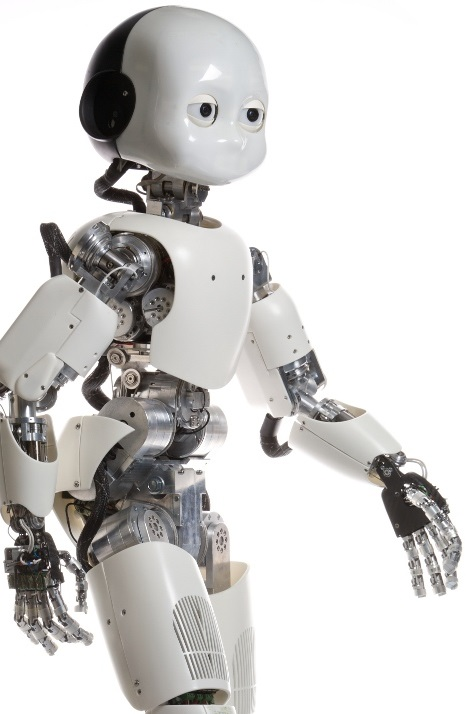
\includegraphics[width=0.85\textwidth]{schemi/icub}
\end{figure}
\end{columns}
\end{frame}

\begin{frame}
\frametitle{Introduction 4/4}
Solutions:
\begin{itemize}
\item Sales of wearable devices;
\item Incrementing chance of having at hand a camera;
\item Incrementing number of images taken every day \cite{photos};
\item Deeper neural networks;
\end{itemize}
\end{frame}
         
\begin{frame}
\frametitle{References}
   \begin{thebibliography}{9}
	\bibitem{photos}
		Caroline Cakebread
		\newblock “People will take 1.2 trillion digital photos this year — thanks to smartphones”
		\newblock Businessinsider.com, 1 September 2017
		\newblock Available at: https://www.businessinsider.com/12-trillion-photos-to-be-taken-in-2017-thanks-to-smartphones-chart-2017-8?IR=T
   \end{thebibliography}
\end{frame}

\begin{frame}
\centering
\frametitle{The End}
\Huge Thank you for your attention!
\break
\break
\break
\break
\large Nicolò Bertozzi
\break
Francesco Bianco Morghet
\break
\break
FPAR Project | MLDL
\break
10 July 2020
\end{frame}

\end{document} 